\documentclass[11pt,onecolumn]{article}
\usepackage{makeidx,times,alltt,graphicx,calc,subfigure}
\usepackage{epstopdf}
\usepackage{xspace}
\usepackage{longtable}
\usepackage{wrapfig}
\usepackage{fancyvrb}
\usepackage{booktabs}
\usepackage{ctable}
\usepackage{multirow}
\usepackage{bigdelim}
\usepackage{ctable}
\usepackage{graphicx}
\usepackage{subfigure}
\usepackage{fancyvrb}
\usepackage{color}
\usepackage{listings}
\usepackage{epsfig,alltt}
\usepackage{graphics}
\usepackage{shortvrb}
%\usepackage[english,ruled,vlined]{algorithm2e}
%\usepackage{latexsym}
%\usepackage{amssymb,amsmath}
%\usepackage[usenames]{color}
\usepackage{setspace}
\usepackage{comment}
%\usepackage{ulem}

\usepackage{listings}
\lstset{fancyvrb=true}
\lstset{
    language=C++,
        basicstyle=\footnotesize\tt,
        %basicstyle=\tt, 
        %keywordstyle=\color{blue},
        identifierstyle=,
        %commentstyle=\color{green},
        %stringstyle=\color{red},
        showstringspaces=false,
        captionpos=t,
        tabsize=3,
        %linewidth=12mm,
        numbers=left, 
        stepnumber=2
}

%\usepackage{pdftricks}
%\begin{psinputs}
%\usepackage{pstricks}
%\usepackage{color}
%\usepackage{pstcol}
%\usepackage{pst-plot}
%\usepackage{pst-tree}
%\usepackage{pst-eps}
%\usepackage{multido}
%\usepackage{pst-node}
%\usepackage{pst-eps}
%\end{psinputs}

%\newcommand{\comment}[1]{}
\newcommand{\charmpp}{\textsc{Charm++}}
\newcommand{\namd}{\textsc{namd}}
\newcommand{\charisma}{Charisma}
\newcommand{\divcon}{\emph{DivCon}}
\newcommand{\openatom}{\textsc{OpenAtom}}
\newcommand{\LeanCP}{\textsc{OpenAtom}}
\newcommand{\leancp}{\textsc{OpenAtom}}
\newcommand{\changa}{ChaNGa}
\newcommand{\kale}{Kale}
\newcommand{\sdag}{Structured Dagger}
\newcommand{\parfum}{{\sc ParFUM}}
\newcommand{\metis}{{\sc Metis}}
\newcommand{\note}[1]{\emph{(Note: #1)}}
\newcommand{\tight}{\baselineskip=8pt}
\newcommand{\etal}{{\em et al.}}
\newcommand{\viz}{{\em viz.}}
\newcommand{\nbody}{$N$-body}
\newcommand{\kdtree}{$k$d-tree}

\def\code#1{{\small {\tt {#1}}}}
\def\smallfbox#1{{\small {\fbox{#1}}}}
\def\porder#1#2#3{$#1 <_{#3} #2$}
\def\lhs#1#2{$#2 \in \mathit{LHS}(#1)$}
\def\rhs#1#2{$#2 \in \mathit{RHS}(#1)$}


\oddsidemargin=-0.25in
\textwidth=7in
\topmargin=-0.25in
\headheight=0in
\headsep=0in
\textheight=9.5in

\begin{document}
%\doublespacing

\title{ ECE598KH Final Project Report \\ NAMD GPU Performance Analysis and Tuning}

\author{
  Yanhua Sun, Xin Zhao\\
  University of Illinois at Urbana-Champaign\\
  \{sun51, xinzhao3\}@illinois.edu
}

\date{}
\maketitle

\lstset{
  basicstyle=\ttfamily,
  showstringspaces=false
}

%\begin{tight}
%\bibliographystyle{abbrv}
%\bibliography{group,cited}
%\end{tight}

\section{Introduction}
In this project, the application we are focusing on is NAMD.
NAMD~\cite{NamdSC02}, recipient of a 2002 Gordon Bell Award, is a parallel molecular 
dynamics code designed for high-performance simulation of large biomolecular systems.
It was developed in the mid-1990's. Now it is one of the most widely used molecular dynamics 
software with more than 50,000 users. It was also selected by NSF as an acceptance test
for Blue Waters.
Through many years, NAMD has been highly optimized to achieve scalable performance on CPU.
It has successfully scaled to the full Titan supercomputer with around $300K$ cores and 
the full Blue Waters with $400K$ cores.

These years, GPU-accelerated algorithms have demostrated speedup of 10- to 100-fold. Meanwhile, 
the hardware has been improved significantly to better match the needs of algorithms over the years.
Since 2006, NAMD has been accommodated to take the advantage of GPU-accelerators. Speedup of 
6- or even 10- has been demonstrated in the previous work~\cite{phillips_stone_namd_cuda}.
Although NAMD GPU has been carefully designed and optimized, it still needs a lot of 
efforts to maximize the performance on GPU, especially on the new hardware such as Fermi, Kepler. 

In this report, we first analyzed NAMD performance on two machines with different configurations.
One is with fast CPU but slow old GPU while the other has fast GPU but slower CPU. We showed 
the results and explained the reasons. Based on our analysis, we optimized the GPU kernel code
to reduce the GPU time. This optimization helps when GPU becomes performance bottleneck.
At the same time, due to the difference of total CPU and GPU capabilities, the load between them
can be imbalanced. We also proposed and implemented a load balancing strategy between CPU and GPU.
We demostrate the effectiveness of our optimizations by comparing the original performance results
and new results.

%\namd{}

\section{NAMD GPU Design } 

Explain computes, patch, nonbonded work  


\section{NAMD GPU CPU Load Balance}
\label{sec:balance}
As we described earlier, in \namd{} GPU design all nonbonded work 
is offloaded to GPU since its computation is most intensive.
In code shown in ~\ref{gpu-cpu-assignment}, it is implemented by assigning computes to GPU so long as 
it has the types of Nonbonded*, which include NonbondedPair and
NonbondedSelf.  

%\begin{lstlisting}[float,frame=single,caption={Compute Assignment},label=gpu-cpu-assignment]
\begin{lstlisting}[frame=single,caption={Compute Assignment},label=gpu-cpu-assignment]
switch ( type of compute )    
{
    case computeNonbondedPairType:
            register_cuda_compute_pair(i,pid2,trans2);
            break
   ........................
   other types:
            create computes on CPU
            break;
}

\end{lstlisting}

\textbf{Motivation} : While this is a straightforward way to balance load between CPU and GPU, 
it may have significant performance problem depending on the configuration
of GPU and CPU.

We first did our experiments on two machines. The first is a multicore desktop with old GTX8800 
GPU and Intel Core2 Quad cores. The other machine is JYC, a test bed of Blue Waters. Each GPU node of 
JYC has 1 Kelper GPU and 16 AMD Interlagos cores. Table~\ref{tab:jac-desktop} shows the time step 
of simulating $23558-atom DHFR$ system on lab machine. It can be seen that the time step 
does not change when we use GPU or not. Moreover, using more CPU cores also does not help improve performance.
This is mainly because GPU is so slow and becomes the bottleneck of the performance.

\begin{table*}
\centering
\begin{tabular}{|c|c|c|c|}
\hline
 configuration & 1 CPU core  & 1 CPU core + 1 GPU & 4 CPU cores + 1 GPU \\
\hline
timestep (ms/step) & 673 & 725 & 720 \\
\hline 
\end{tabular}
\caption{Simulating 23558 atoms DHFR on desktop}
\label{tab:jac-desktop}
\end{table*}

Table~\ref{tab:jac-JYC} shows the time step of simulating $92224-atom Apoa1$
using one node of JYC. In the cases of using only one CPU core and one CPU core 
plus one GPU core, using GPU provides a speedup of 8.4x. 
Also when we increase the number of CPU cores upto 15, 
 the speedup is almost 40x.   

\begin{table*}
\centering
\begin{tabular}{|c|c|c|c|}
\hline
 configuration & 1 CPU core  & 1 CPU core + 1 GPU & 15 CPU cores + 1 GPU \\
\hline
timestep (ms/step) & 990 & 117 & 25 \\
\hline 
\end{tabular}
\caption{Simulating 92224 atoms Apoa1 using one node of JYC }
\label{tab:jac-JYC}
\end{table*}


To better understand the performance change in table~\ref{tab:jac-JYC},
we plot timelines of CPU and GPU execution. 
Fig.~\ref{figs:gpu-ppn1} and ~\ref{figs:gpu-ppn15} show the timeline of 
running $92,224$ atom Apoa1 using 1 GPU and 1 CPU core, 1GPU and 15 CPU cores.
Each main line represents execution on one CPU core. Different colors stand for 
different function execution. The red activity is for integration while the purple
is all bonded work on CPU. The white color stands for idle time. The green bars on top of the main bars 
show the execution of GPU. In Fig.~\ref{figs:gpu-ppn1}, the total time range 
is around $117 ms$, which is the time for one simulation step. We can see that
GPU only takes a small portion of total time, which is around $19 ms$.
In this case, it is correct that we should offload as much nonboned work as possible
to GPU since CPU execution is relatively slow. 

However, in Fig.~\ref{figs:gpu-ppn15} when we increase the number of CPU cores, 
the work on CPU side is parallelized and time is reduced to $12 ms $ while the GPU exection
still takes $19 ms$. As a result, on CPU side, there is a big portion of idle time.    

\begin{figure}[h]
\centering
\subfigure[1CPU core + 1 GPU] {\label{figs:gpu-ppn1}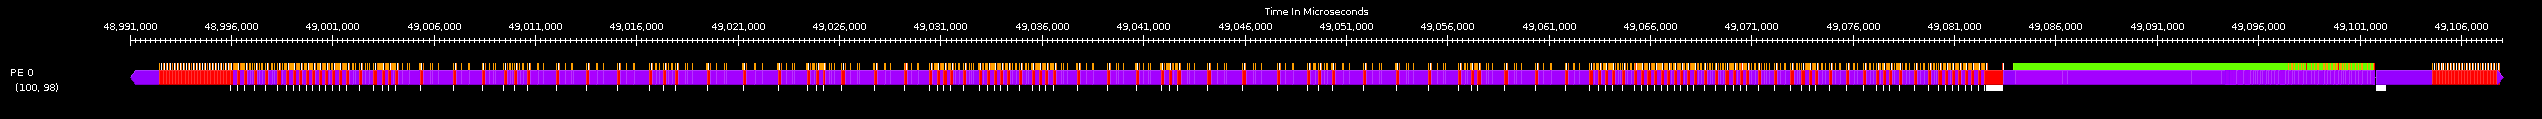
\includegraphics[width=5.8in]{figs/gpu-ppn1-timeline-117ms.png}}
\subfigure[15 CPU cores + 1 GPU] {\label{figs:gpu-ppn15}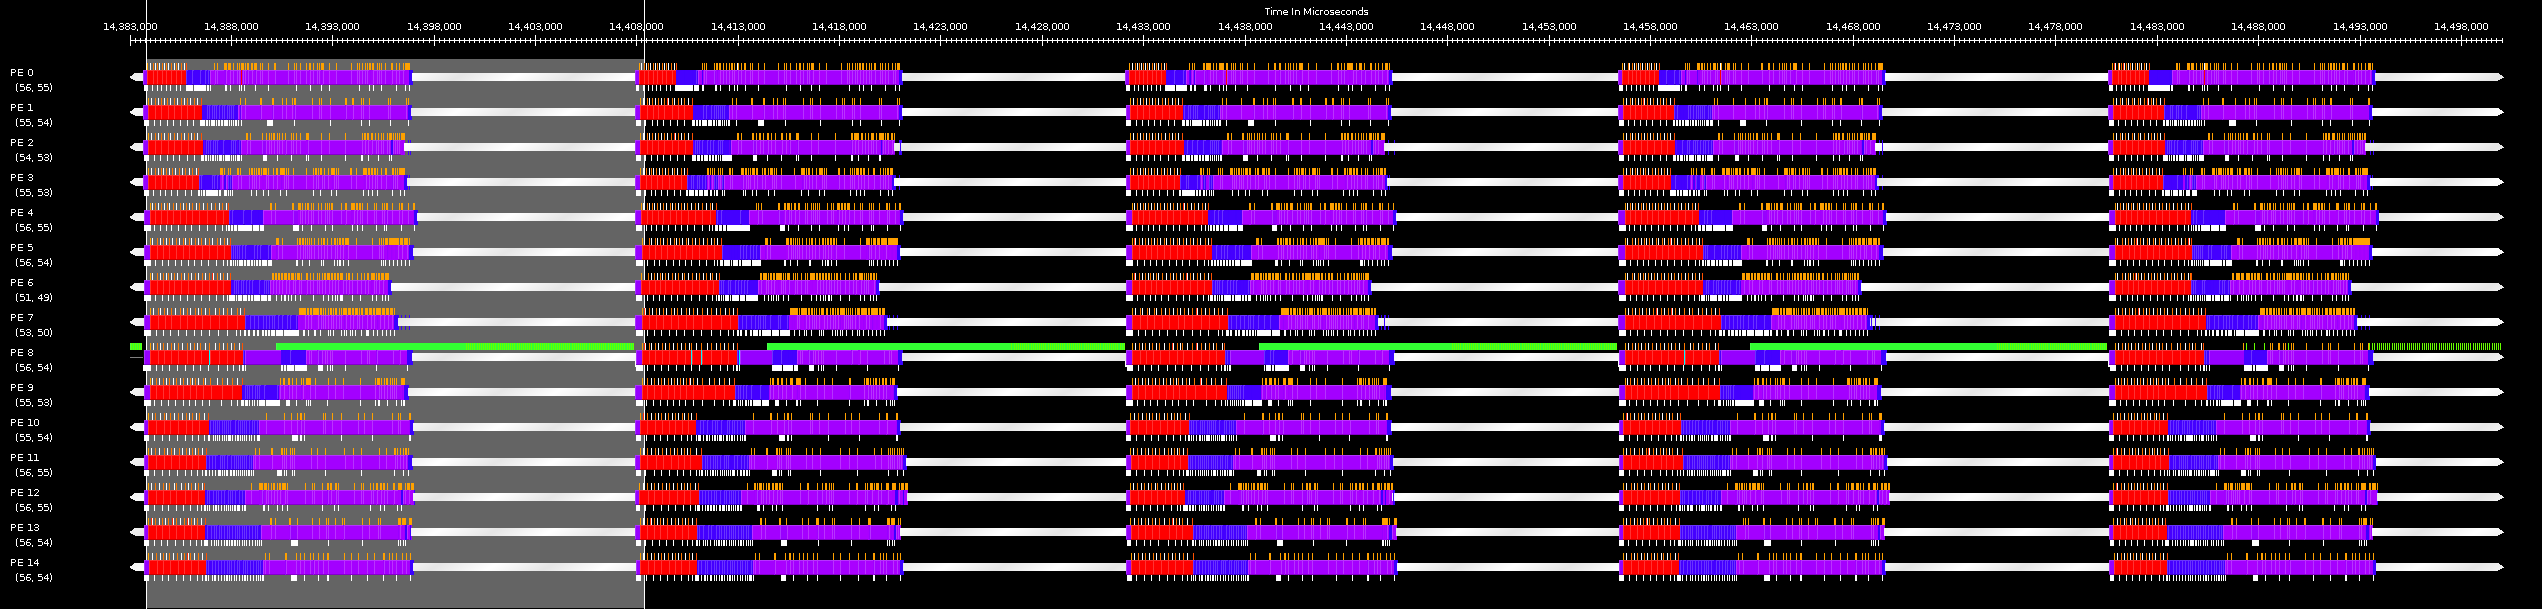
\includegraphics[width=5.8in]{figs/gpu-ppn15-timeline-117-25ms.png}}
\caption{Timeline of running Apoa1 with 1 GPU and different number of CPU cores}
\label{figs:cpu-gpu}
\end{figure}

\textbf{Load Balance} From table~\ref{tab:jac-desktop}, we can conclude that 
to calculate the same amount of nonboned work, the speed of GPU to CPU is 
$673:725 = 9:10$. Therefore, when one CPU core and one GPU is used, 
    the ratio of their nonboned work is roughly $10:9$. When using multiple CPU cores,
    the ratio of CPU and GPU work should be  $10*cores : 9 $.

In table~\ref{tab:jac-JYC}, when using one CPU core, the time to calculate nonboned work 
is  $ 990-117 = 873$. When all nonboned work is offload to GPU, the time cost is 
$18$ as shown in green bars in Fig.~\ref{figs:cpu-gpu}. Therefore, the ration of GPU 
and CPU capability is $873:18 = 48:1$. Since we have multiple CPU cores, the ratio of work on CPU 
and GPU should be $ Cores: 48 $.

Currently, we hard code this ratio into code. In future, we plan to use more intelligent instrumentation-based
balance scheme. Now with balance scheme, when we assign work, we need to figure out 
whether a compute should be placed on GPU or CPU. The changed code is as follow:

\begin{lstlisting}[frame=single,caption={Balanced Compute Assignment},label=gpu-cpu-assignment-balance]
switch ( type of compute )    
{
   case computeNonbondedPairType:
     if(computeid % ratio  < GPUload)
         register_cuda_compute_pair(i,map->computeData[i].pids[0].pid);
     else
     {
         c = new ComputeNonbondedPair(i,map->computeData[i].pids[0].pid,
             computeNonbondedWorkArrays,
             map->partition(i),map->partition(i)+1,
             map->numPartitions(i)); // unknown delete
            //assign work on CPU
            map->registerCompute(i,c);
            c->initialize();
       }
     break;

     other types:
         create computes on CPU
         break;
}
\end{lstlisting}

%\section{Background}
%In a molecular dynamics simulation, a collection of atoms interact through a set of forces. 
%Since each atom interacts with all the other atoms, the complexity of calculating forces
%is $O(Atoms^2)$. This algorithm does not scale with the number of atoms. Based on the fact that
%atoms from far distance contribute little to the force calculation, in \namd{} the interaction is
%calculated by short range forces and long range forces. The molecule  is spatially divided into 
%patches based on cutoff distance. Atoms in one patch only interact with other atoms in neighbor patches.
%To be more accurate, long range electrostatics calculation is performed through particle-mesh Ewald (PME) method.
%For these two types of calculation, short range forces are computation intensive while PME is communication intensive.
%Therefore, in current NAMD GPU design and implementation, non-bonded cutoff computation is offload to GPU.
%All other bonded work, integration and PME work is remained on CPU.

%\section{Objective}

\section{NAMD GPU Kernel Optimization}
\subsection{GPU Force Calculation Kernel}

In the original GPU kernel implementation, each thread block calculates the forces on the atoms in one patch (patch 1)
due to the atoms in another patch (patch 2). Fig.~\ref{figs:pseudocode} presents the pseudo-code for kernel calculation.
In the outer loop, each thread copies atoms from patch 1 to local registers. In the inner loop. threads in the block collaborate to
load atoms from patch 2 to shared memory. Before and after reading of atoms in patch 2, there are synchronization calls to guarantee
that data is ready to be used before the calculation and is ready to be rewritten after the calculation. During the force
calculation phase, each thread iterates atoms in patch 2 and computes the distance with current atom in patch 1.
If the distance is within cut-off distance, it accumulates the forces for the current atom in patch 1 and finally writes force results
back to GPU global memory. The kernel also calculate a pairlist every 10 time steps used by following time steps to further avoid redundant work. 

\begin{figure}[h]
\centering
\setlength{\abovecaptionskip}{-1pt}
\setlength{\belowcaptionskip}{-2pt}
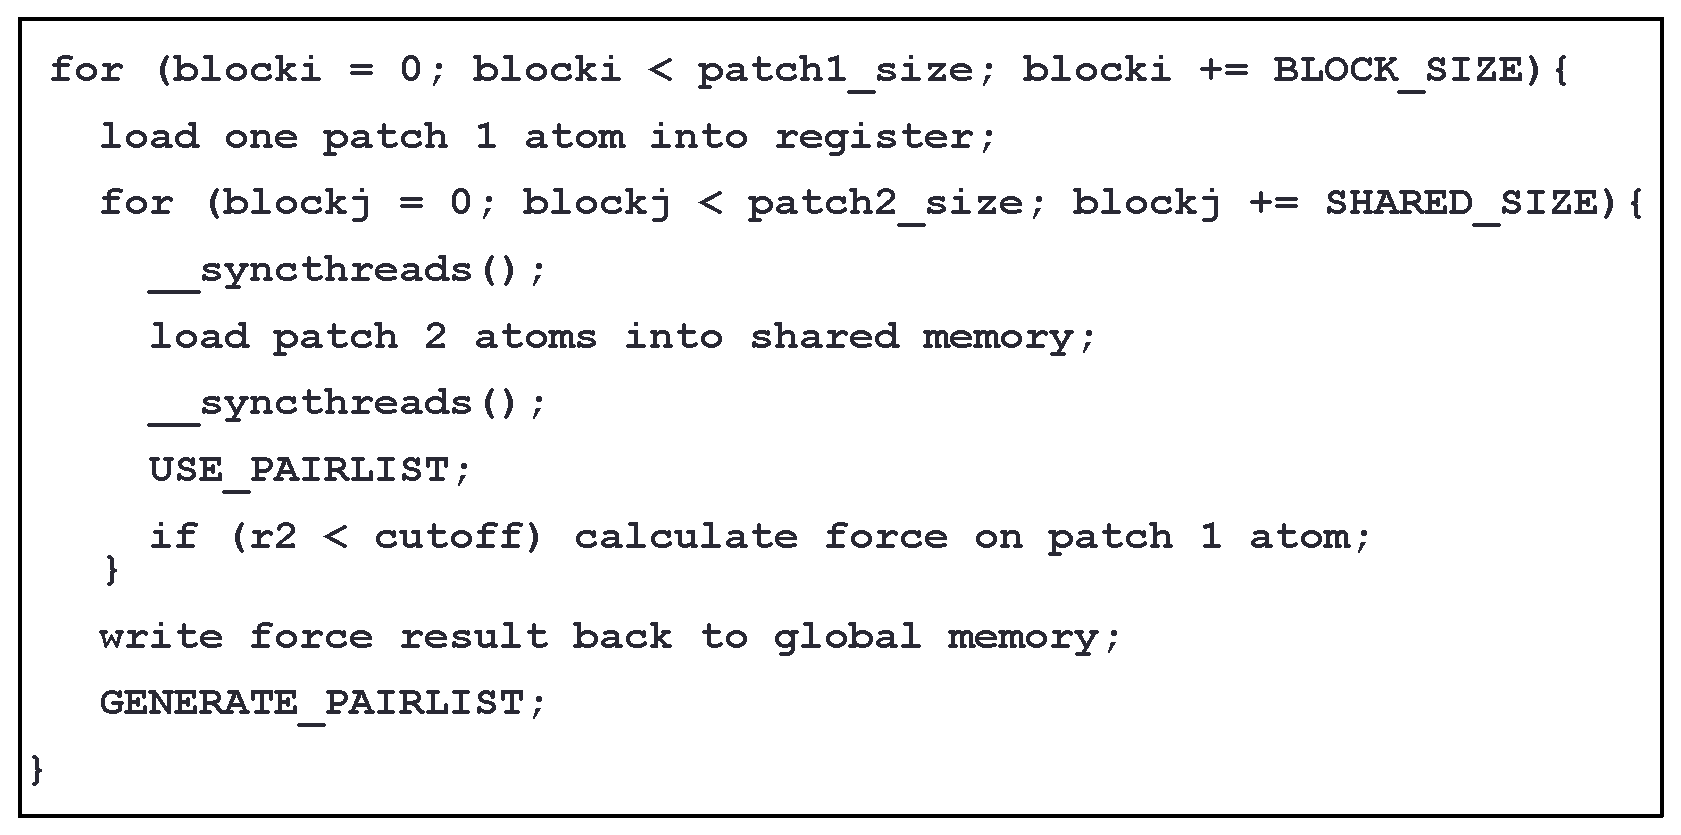
\includegraphics[width=4.0in]{figs/pseudocode.eps}
\caption{Pseudocode for GPU kernel force calculation}
\label{figs:pseudocode}
%\vspace{-0.5cm}
\end{figure}

After profiling the performance of the GPU kernel, we acquired the following observations:
(1) force calculation dominates the most GPU time compared to data loads and stores;
(2) there are great control divergence among different threads due to thread synchronization, which means some threads take a really long time
to reach the synchronization where other threads reach it very quickly. However, all threads in the block have to wait for everyone to
reach the synchronization before they can process further. Besides, use of pairlist may aggravate the divergence.
Based on above observations, we proposed several optimization approaches to reduce the control
divergence. They are described in detail in following sections.

\subsection{Optimizations}
\subsubsection{Patch 1 Atoms Tiling}

As indicated in Fig.~\ref{figs:pseudocode}, in each outer loop, for one atom in patch 1, every thread needs to iterate and examine all loaded atoms from patch 2
and call synchronization routines. In order to reduce the synchronization overhead, we first considered tiling of patch 1 atoms,
in which every thread loads mulitple atoms instead of only one atom from patch 1 in each outer loop.
By doing this, total number of outer loops can be reduced. Furthermore, data reuse of patch 2 is improved because now atoms from patch 2 is used to calculate
forces of more atoms from patch 1.

Fig.~\ref{figs:divergence} shows an example of how merging loops can improve the performance. Suppose thread 1 (T1) has 9 units of computation in the first loop and 2 units
of computation in the second loop, whereas thread 2 (T2) has 3 units to do in the first loop and 8 units to do in the second loop. In the first loop T2 needs to wait for
completion of T1 while in the second loop T1 needs to wait for T2. Both threads have to spend long time waiting for each other and total synchronization time is 17.
After merging loops on both T1 and T2, divergence between them is reduced, synchronization call is decreased by 1, and now total synchronization time is 11.

\begin{figure}[h]
\centering
\setlength{\abovecaptionskip}{-1pt}
\setlength{\belowcaptionskip}{-5pt}
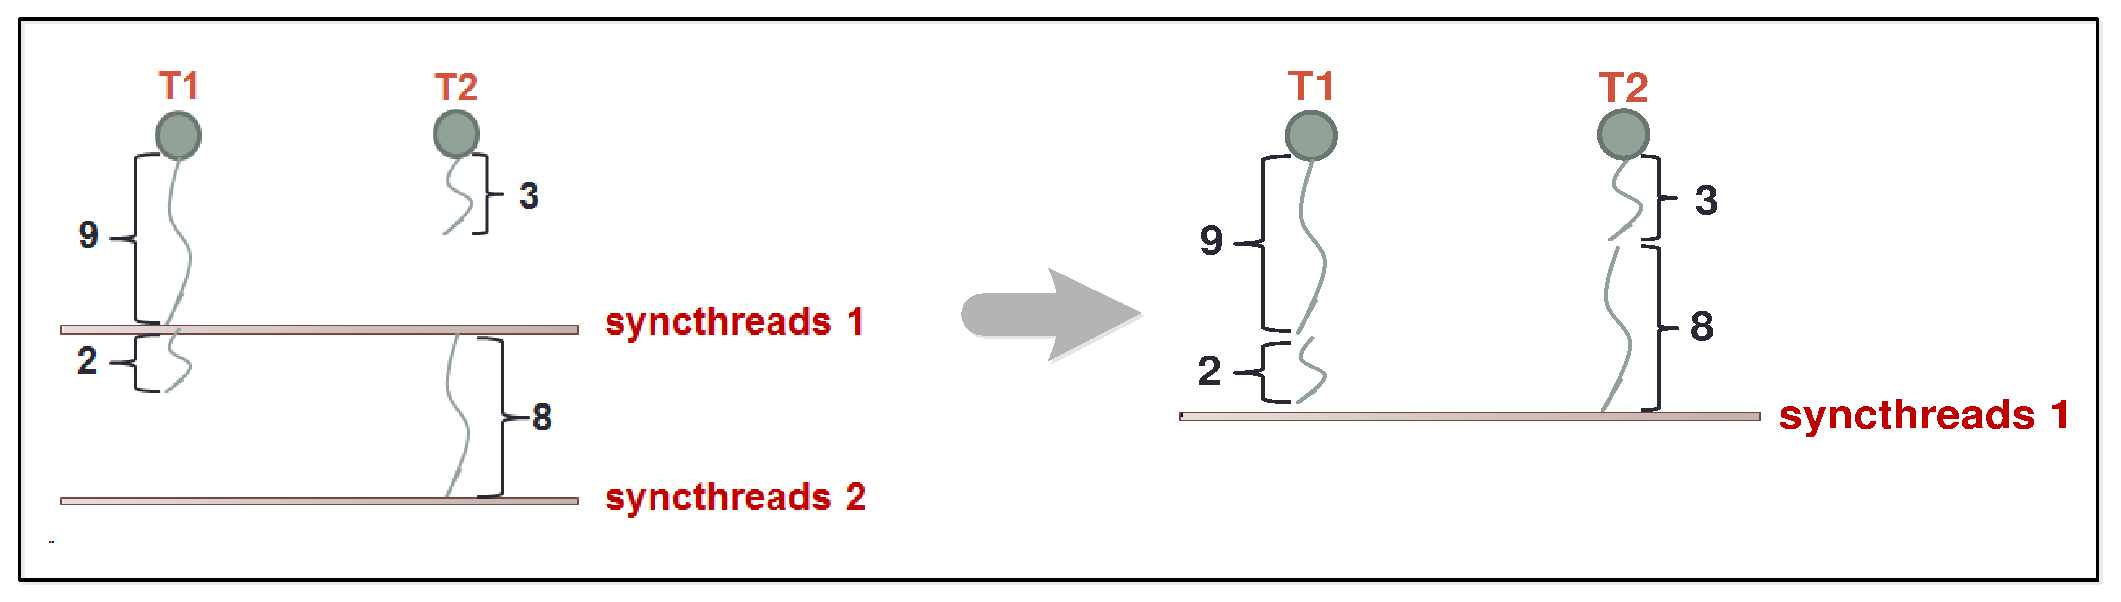
\includegraphics[width=6.0in]{figs/divergence.eps}
\caption{Reduce control divergence by merging loops}
\label{figs:divergence}
\vspace{-0.5cm}
\end{figure}

\subsubsection{Patch 2 Atoms Tiling}

After finishing tiling of loading patch 1 atoms, we consider tiling of loading patch 2 atoms to further reduce synchronization calls.
In the original implementation in Fig.~\ref{figs:pseudocode}, for each inner loop, all threads in the thread block collaborate to load SHARED\_SIZE
patch 2 atoms for just one time.
In our optimization, we make all threads load patch 2 atoms multiple times with SHARED\_SIZE in each time. Fig.~\ref{figs:pseudocode-tile} shows
the pseudo-code after tiling is applied. TILE\_WIDTH\_1 and TILE\_WIDTH\_2 are macros to set tile widths for patch 1 and patch 2 correspondingly.

\begin{figure}[h]
\centering
\setlength{\abovecaptionskip}{-1pt}
\setlength{\belowcaptionskip}{-2pt}
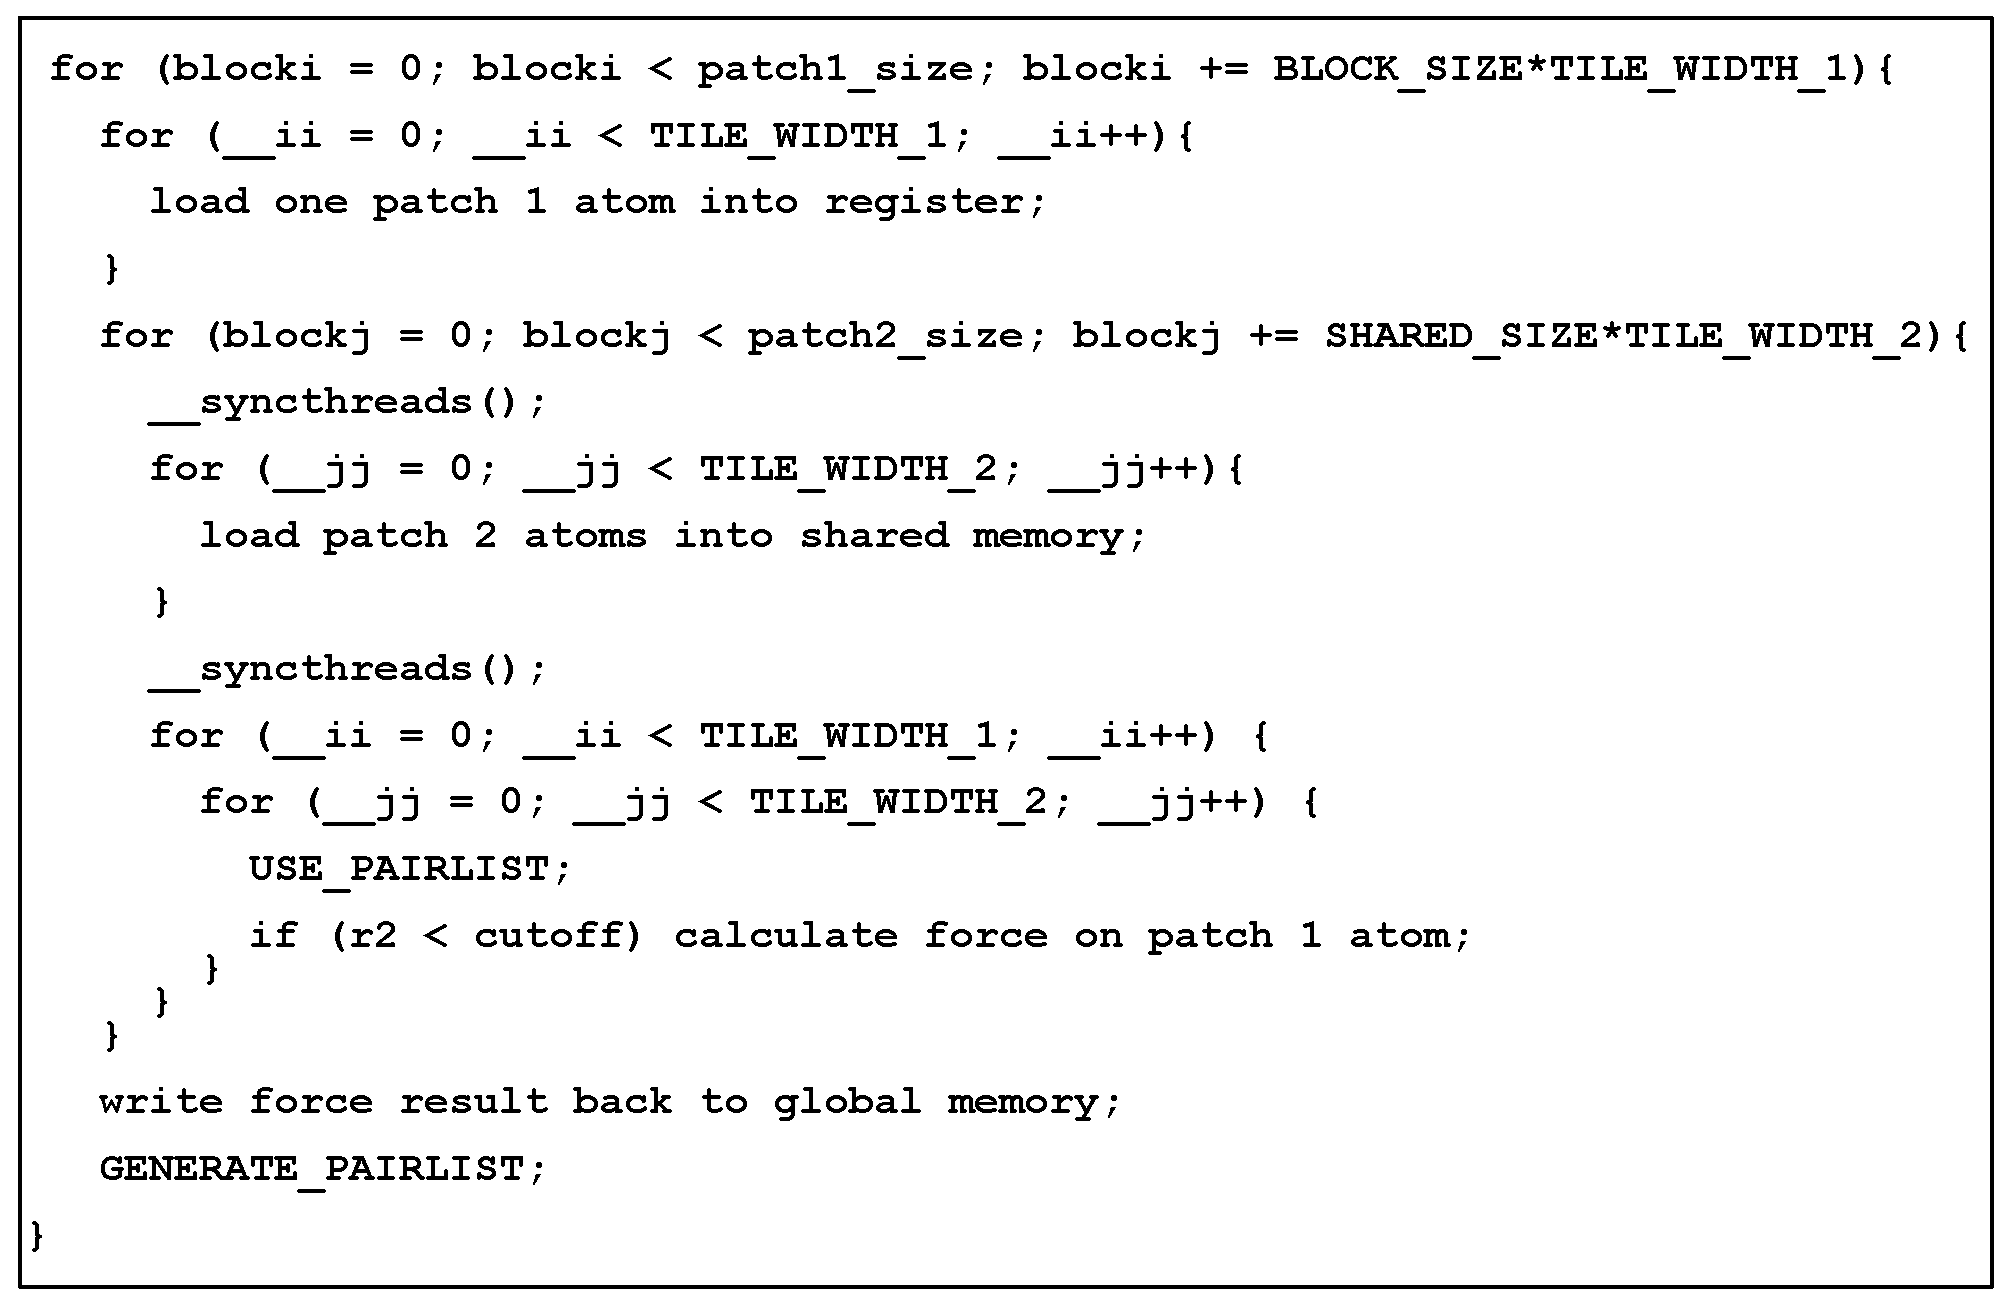
\includegraphics[width=4.0in]{figs/pseudocode-tile.eps}
\caption{Pseudocode for GPU kernel force calculation after tiling optimization}
\label{figs:pseudocode-tile}
%\vspace{-0.5cm}
\end{figure}

Fig.~\ref{figs:patch1-count} shows a comparison of computation time among different patch 1 atoms, which is derived by examining a system with 401 atoms in patch 1
and counting how many inner loop needed for each atom. Because there are 401 atoms in total and 128 threads in one thread block, it needs four outer loops to
complete the work. In Fig.~\ref{figs:patch1-count}, region between read dashed lines represents work on atoms assigned to the first
warp and red circles indicate the maximum computation time in current outer loop. The sum results of four read circles is about 920, which indicates
the total work time for the first warp when inner loop is completely tiled and outer loop is not (one synchronization in each outer loop).

Fig.~\ref{figs:thread-count} shows a comparison of computation time among different threads within one thread block, by examining the same system
in Fig.~\ref{figs:patch1-count}. Similarly, region betwen read dashed lines represents work on the first warp. It is shown that the maximum computation time
in this figure is below 800. It inidcates the total work time for the first warp when both inner loop and outer loop are completely tiled (only one synchronization exists). 

\begin{figure}[h]
\centering
\setlength{\abovecaptionskip}{-1pt}
\setlength{\belowcaptionskip}{-2pt}
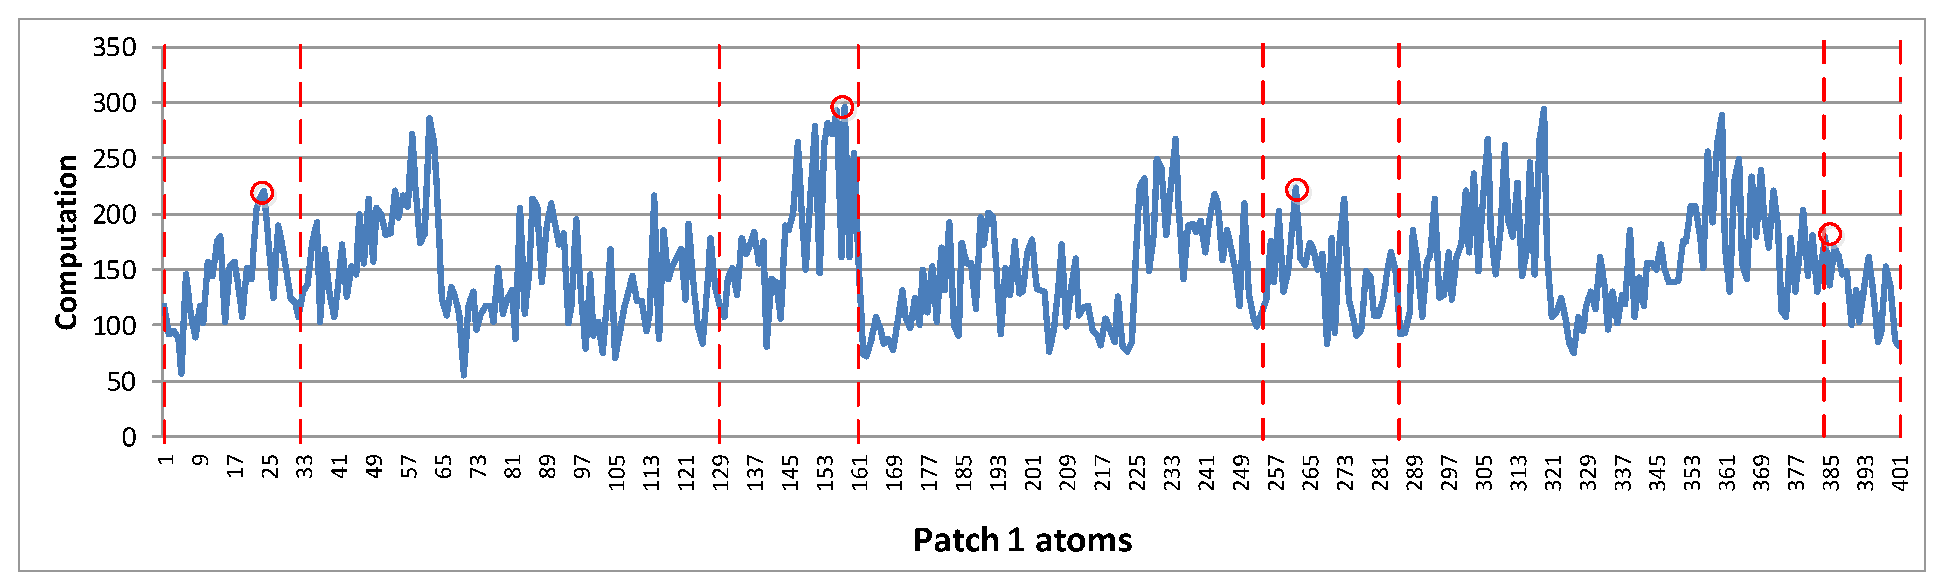
\includegraphics[width=6.0in]{figs/patch1_count.eps}
\caption{Computation comparison for different patch 1 atoms}
\label{figs:patch1-count}
\vspace{-0.5cm}
\end{figure}

\begin{figure}[h]
\centering
\setlength{\abovecaptionskip}{-1pt}
\setlength{\belowcaptionskip}{-2pt}
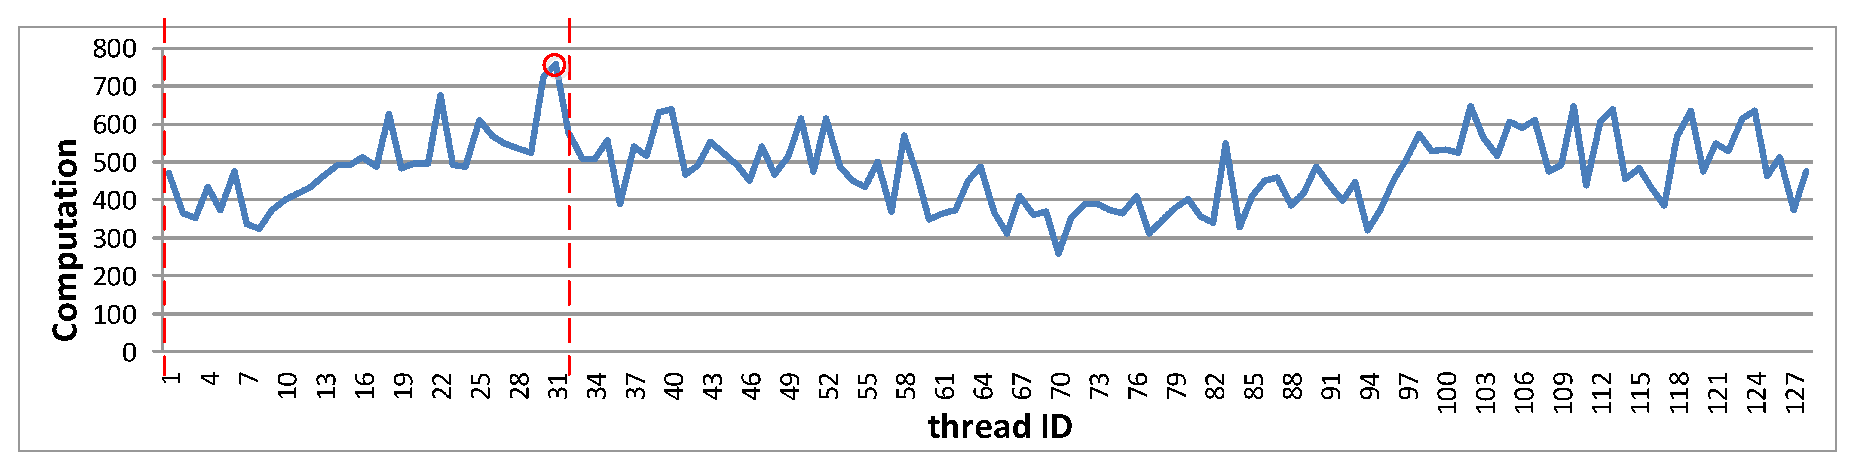
\includegraphics[width=6.0in]{figs/thread_count.eps}
\caption{Computation comparison for different threads}
\label{figs:thread-count}
\vspace{-0.5cm}
\end{figure}

\subsubsection{Patch 1 Atoms Sorting}

Inspite of merging loops, we observe that control divergence still exists because there are some threads that always have large work and some threads
that always have small work in each loop. In this case, merging loops would not make a big difference since threads still have to wait for those with
large work to finish. To reduce the control divergence, an effective optimization approach is assigning patch 1 work in a more regular way.
In each time step, we first sort the patch 1 atoms according to their workload, and then pass the sorting result to the next time step to assign the work to threads.
By assigning patch 1 atoms based on sorting instead of randomly, work differences among threads within one warp is not as large as before, and large work
are all assigned to the last warps. The workload on atoms is not changed very little between consecutive time steps, therefore sorting result from the last time step
can be applied to the current time step. 


\section{Performance Results}
   


\section{Conclusion and Discussion}
 


\bibliographystyle{abbrv}
\bibliography{group,cited}
\end{document}


